% !TEX root = ../my-thesis.tex
%
\chapter{State of the Art}
\label{sec:sota_1}

\cleanchapterquote{All models are wrong, but some are useful.}{ George E. P. Box,}{(British Statistician, 1919-2013)}


\section{Calibration of Computer Codes: Frequentist and Bayesian Perspectives}
\label{sec:sota_1:bayesian_calibration}


A model is a tool used by scientists and engineers to understand and predict the world by mathematically describing different phenomena. Mathematical models encode the behavior of a physical system in a mathematical form, which are then implemented and solved using numerical methods on a computer code. In this work, we mainly investigate models that transform some input conditions $\bx \in \mathrm{X} \subset \reals^{d_x}$ into a scalar \gls{qoi} $y \in \mathrm{Y} \subset \reals$. These models are parameterized by some parameters $\btheta \in \Theta \subset \reals^{d_p}$. These parameters can be physical measurable quantities, like physical constants, or tuning parameters, that lack physical meaning. The relationship between these quantities shall be expressed as,

\begin{equation}
    y = f(\bx; \btheta)\;.
    \label{eq:sota_1:y}
\end{equation}

where $f(.;.) : \mathrm{X} \times \Theta \rightarrow \mathrm{Y}$ is a computer model. The process of computing the \gls{qoi} $y$ given an input condition $(\bx;\btheta)$ is called \textit{evaluation} while the process of inferring the value of the parameters $\btheta$ given some data $\data = \{(\bx_i,y_i)\}_{i=1}^{\nobs}$ is called \textit{calibration}~\cite{uq_theory} and is the primary interest of this work. Calibration can be used to build surrogate models, with $\data$ corresponding to a set of evaluations of a (possibly complex or expensive) code and $\btheta$ to a set of tuning parameters~\cite{Banks1989}. Calibration is also used to reconstruct unmeasurable physical quantities~\cite{params_cali}, $\btheta$, with $\data$ now corresponding to a set of measurements \blue{of the physical process that the numerical solver $f$ represents}. In this work, we will focus on the latter case, in which $\btheta$ corresponds to some physical parameters that we want to infer from data $\data$.

\begin{figure}[htbp]
  \centering
  \begin{subfigure}[t]{0.7\linewidth}
    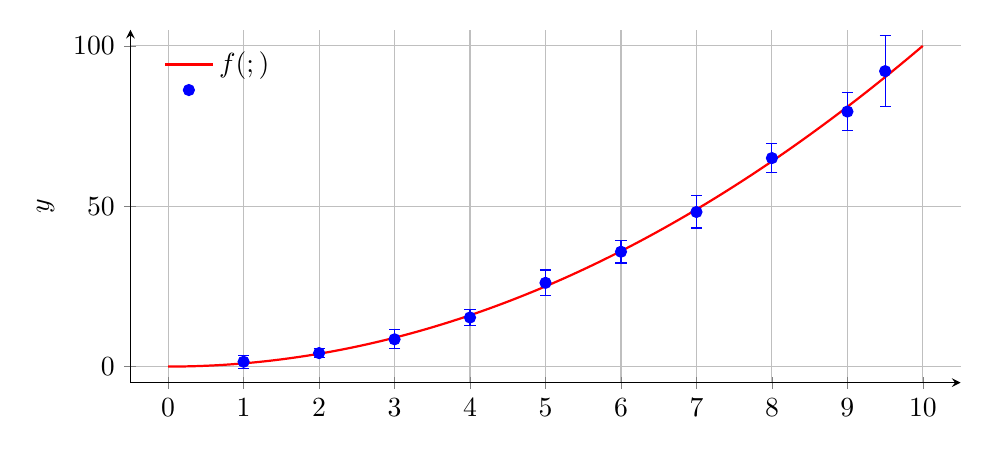
\begin{tikzpicture}
        \begin{axis}[
            % Dimensions to make it span the text width and be roughly 1/6th tall
            width=\textwidth,
            height=0.50\textwidth, 
            % Axis labels
            xlabel={$\bx$},
            ylabel={$y$},
            % Legend placement and style
            legend pos=north west,
            legend style={draw=none, fill=none},
            % Grid and axis styling
            grid=major,
            axis lines=left,
            xmin=0, xmax=10,
            ymin=0, ymax=100,
            enlargelimits=0.05
        ]

        % 1. The Model (Continuous Curve)
        % Using a simple quadratic curve (y = x^2) as a dummy model
        \addplot [
            domain=0:10,
            samples=100,
            color=red,
            thick
        ] {x^2};
        \addlegendentry{$f(\bx;\btheta)$}

        % 2. Experimental Data (Points with Error Bars)
        \addplot [
            only marks,
            color=blue,
            mark=*,
            error bars/.cd,
            y dir=both,
            y explicit
        ] coordinates {
            % Format: (x, y) +- (0, y-error)
            (1, 1.5) +- (1.3, 2.0)
            (2, 4.2) +- (2.5, 1.5)
            (3, 8.5) +- (3.5, 3.0)
            (4, 15.3) +- (4.5, 2.5)
            (5, 26.1) +- (5.5, 4.0)
            (6, 35.8) +- (6.5, 3.5)
            (7, 48.2) +- (7.5, 5.0)
            (8, 65.0) +- (8.5, 4.5)
            (9, 79.5) +- (9.5, 6.0)
            (9.5, 92.1) +- (10.5, 11.0)
        };
        \addlegendentry{$\data$}

        \end{axis}
    \end{tikzpicture}
    \caption{Calibration curve comparing the computer model against experimental data points.}
    \label{fig:calibration_1}
  \end{subfigure}
  \begin{subfigure}[t]{0.7\linewidth}
    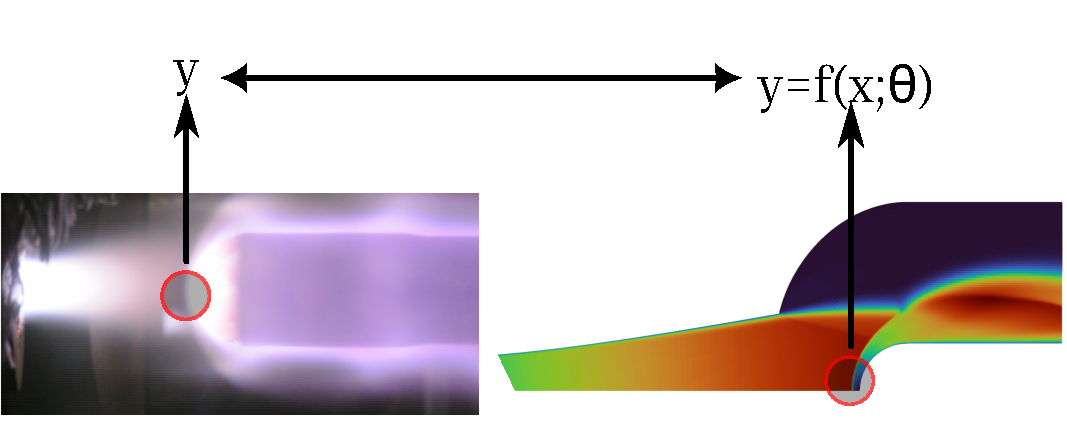
\includegraphics[width=\textwidth]{figures/sota_1/calibration.pdf}
    \caption{Schematic representation of an experiment and a corresponding computer code.}
    \label{fig:calibration_2}
  \end{subfigure}
  \caption{\blue{Visual representation of the calibration process, illustrating the comparison between a computer model and experimental data, as well as the relationship between an experiment and its corresponding computer code.}}
  \label{fig:sota_1:cali}
\end{figure}


Fig.~\ref{fig:sota_1:cali} intuitively describes the process of calibration: \blue{Fig.\ref{fig:calibration_1} shows a calibration curve, where the theoretical model $f(\bx;\btheta)$ is compared against experimental data points $\data$. The goal of calibration is to adjust the parameters $\btheta$ such that the model output aligns closely with the observed data. Fig.~\ref{fig:calibration_2} provides a schematic representation of an experiment and its corresponding computer code, illustrating an experiment of a high enthalpy jet impinging on a probe and the corresponding computer code that simulates the same physical phenomenon. The calibration process involves adjusting the parameters of the computer code to match the experimental observations, thereby improving the accuracy and reliability of the model.} In this work, we will focus on the case in which the data $\data$ is affected by some noise $\epsilon(\bx)$, which can be due to measurement errors or other sources of uncertainty. In this case, we can write,

\begin{equation}
    y = f(\bx;\btheta) + \epsilon(\bx) \;.
    \label{eq:sota_1:nme}
\end{equation}

Note that Eq.~\eqref{eq:sota_1:nme} is valid in the case of additive noise, expressions for multiplicative noise can be found in~\cite{mult_noise}. Eq.~\eqref{eq:sota_1:nme} is written for a single observation, but in practice we have access to a whole dataset $\data = \{(\bx_i,y_i)\}_{i=1}^{\nobs}$. We can therefore upgrade Eq.~\eqref{eq:sota_1:nme} to the vector form,

\begin{equation}
    \mathbf{y} = f(\mathbf{X};\btheta) + \boldsymbol{\epsilon} \;.
    \label{eq:sota_1:nme_vector}
\end{equation}

where $\mathbf{y} = (y_i)_{i=1}^{\nobs}$, $\mathbf{X} = (\bx_i)_{i=1}^{\nobs}$, and $\boldsymbol{\epsilon} = (\epsilon(\bx_i))_{i=1}^{\nobs}$. We further assume that $\boldsymbol{\epsilon}$ is centered Gaussian $\boldsymbol{\epsilon} \sim \normalpdf(\boldsymbol{0}, \boldsymbol{\Sigma}_e)$ (see \cite{data_inconsistency,uq_theory} for more general expressions) with $\boldsymbol{\Sigma}_e$ the covariance matrix of the measurement noise. \blue{The presence of experimental noise $\boldsymbol{\epsilon}$ makes the calibration task challenging, as it prevents the data $\data$ from being perfectly explained by the model $f(\mathbf{X};\btheta)$, no matter the value of $\btheta$. To address this, one common approach is to find the value of $\btheta$ that minimizes the distance between the observed data and the model output, taking into account the noise characteristics. This leads to an optimization problem where we seek to minimize the discrepancy between the model predictions and the noisy observations.}

\begin{equation}
    \hat{\btheta} = \argmin_{\btheta \in \Theta} \| \mathbf{y} - f(\mathbf{X};\btheta) \|^2_{\boldsymbol{\Sigma}_e} \;.
    \label{eq:sota_1:ols}
\end{equation}

where $\|\cdot\|_{\boldsymbol{\Sigma}_e}$ is the distance induced by the covariance matrix $\boldsymbol{\Sigma}_e$. This is the classical \textit{frequentist approach}~\cite{freq_calibration}, in which the parameters are considered as deterministic but unknown values and the goal is to find a single value $\hat{\btheta}$ that best explains the data. The frequentist approaches can be formalized by looking at the \textit{likelihood} of the data given the parameters $\btheta$. The likelihood encodes the probability of actually observing the set of data $\data$ given the parameters $\btheta$. In the case of Gaussian noise, the likelihood reads,

\begin{equation}
    \left. 
        \begin{aligned}
            \likelihood{\data \mid \btheta} &= \normalpdf(\mathbf{y}; f(\mathbf{X};\btheta), \boldsymbol{\Sigma}_e)\\
            &\propto \exp \left( -\frac{1}{2} \|\mathbf{y} - f(\mathbf{X};\btheta)\|_{\boldsymbol{\Sigma}_e}^2 \right) \;.
        \end{aligned}
    \right.
\end{equation}

Under this formulation, the \gls{mle} corresponds to the value of $\btheta$ that maximizes the likelihood, which is equivalent to the value of Eq.~\eqref{eq:sota_1:ols} (precisely because of the Gaussian noise assumption)~\cite{Golberg2010,Seber2005}. The \gls{mle} $\hat{\btheta}$ is actually a random variable since it depends on the data $\data$, which is random even if $\btheta$ is not. Under various assumptions, we can build confidence intervals and asymptotic distributions for $\hat{\btheta}$, which are the bread and butter of Machine Learning and Frequentist statistics~\cite{freq_calibration,uq_theory}.

\smallskip
In a nutshell, in the frequentist framework, the parameters $\btheta$ are considered as deterministic but unknown values and using random data $\data$ we build random estimators $\hat{\btheta}$. It is pedagogical to note that the \gls{mle} estimator is not the only possible estimator, even under the Gaussian noise assumption. Most estimators solve a modified version of the optimization problem in Eq.~\eqref{eq:sota_1:ols}, \blue{which writes:}

\begin{equation}
    \hat{\btheta} = \argmin_{\btheta \in \Theta} \|\mathbf{y} - f(\mathbf{X};\btheta)\|_{\boldsymbol{\Sigma}_e}^2 + R(\btheta) \;.
    \label{eq:sota_1:regularized_ols}
\end{equation}

where $R(\btheta)$ is a regularization function that encodes some \textbf{prior or personal belief} on the parameters $\btheta$. For example, if $R(\btheta) = \lambda \|\btheta\|_2^2$, the estimator is called Ridge Regression; if $R(\btheta) = \lambda \|\btheta\|_1$, the estimator is called Lasso Regression~\cite{BEDOUI2020106917}.

\bigskip
A completely different philosophy is adopted by the \textit{Bayesian framework}, in which the parameters $\btheta$ are themselves random variables. While this might seem at odds with the physical interpretation of $\btheta$ as some physical quantity, it is important to note that the randomness of $\btheta$ is not a property of the parameters themselves but rather a property of our knowledge of those parameters. In other words, the parameters $\btheta$ encode our knowledge of the physical parameters that we are trying to infer. This knowledge is encoded into a probability distribution, which is termed the \textit{prior} distribution $\prior{\btheta}$. The prior encodes all the knowledge and beliefs that we have on the parameters $\btheta$. Notice that in this setting, it makes sense to talk about statistical properties of $\btheta$ such as its mean, variance, or quantiles (exactly like the frequentist talks about the statistical properties of the estimator $\hat{\btheta}$). The data $\data$ is also random and can be used to update our knowledge of the parameters $\btheta$ into a new distribution, called the \textit{posterior} distribution $\p{\btheta \mid \data}$. The posterior distribution encodes all the information that we have on the parameters $\btheta$ after observing the data $\data$. This update is performed using Bayes' theorem, which states that the posterior distribution is proportional to the product of the likelihood and the prior,

\begin{equation}
    \p{\btheta \mid \data} = \dfrac{\p{\data \mid \btheta}\, \prior{\btheta}}{\p{\data}} \;.
    \label{eq:sota_1:bayes}
\end{equation}

Eq.~\eqref{eq:sota_1:bayes} contains the already-mentioned likelihood $\p{\data \mid \btheta}$ and the \textit{evidence} $\p{\data} = \int_{\Theta} \p{\data \mid \btheta} \prior{\btheta} \, \dd\btheta$. The evidence \blue{ensures that the posterior integrates to $1$}. We note that its computation is not necessary to extract samples from the posterior, see \S~\ref{sec:ntools:mcmc}, but \blue{computing it is} crucial for Bayesian model selection techniques~\cite{comp_stat,50_shades_of_bms}. To draw some parallels with the frequentist framework, the \gls{map} value corresponds to the value of $\btheta$ that maximizes the posterior distribution. If we write this optimization problem in the log space, we obtain,

\begin{equation}
   \hat{\btheta} = \argmax_{\btheta \in \Theta} -\frac{1}{2} \|\mathbf{y} - f(\mathbf{X};\btheta)\|_{\boldsymbol{\Sigma}_e}^2 + \log \prior{\btheta} \;.
    \label{eq:sota_1:map}
\end{equation}

Notice the similarity between Eq.~\eqref{eq:sota_1:map} and Eq.~\eqref{eq:sota_1:regularized_ols}. The only difference is that the regularization term $R(\btheta)$ is replaced by the log of the prior $\log \prior{\btheta}$. This is not a coincidence, since as hinted before, the regularization term can be interpreted as a prior belief on the parameters $\btheta$. The \gls{map} value is therefore a special case of the Bayesian framework, in which we only look at the mode of the posterior distribution. 

\smallskip
Although the two approaches share striking similarities, the Bayesian framework is more general and provides a richer description of the parameters $\btheta$ by encoding all the information that we have on those parameters into a probability distribution. For this reason, the Bayesian framework is often preferred in the context of calibration, since it yields a more natural way to quantify and treat the uncertainty on the parameters $\btheta$~\cite{uq_theory}. For example, in uncertainty propagation, one is interested in computing a statistic of a quantity $g(\cdot)$ that depends on the parameters $\btheta$, i.e., $g = g(\btheta)$. In the Bayesian framework, the distribution of $g(\btheta)$ is exactly the push-forward measure of the posterior distribution of $\btheta$ through $g$, denoted as $\mathbb{P}_g = g_{\#}\mathbb{P}_{\btheta \mid \data}$. In terms of densities, this marginal posterior distribution $\p{g \mid \data}$ is obtained by integrating out $\btheta$:
\begin{equation}
  \p{g \mid \data} = \int_{\Theta} \delta\big(g - g(\btheta)\big) \p{\btheta \mid \data} \, \dd\btheta\;,
\end{equation}
which offers a natural and exact mechanism to propagate parametric uncertainty into the quantity of interest. In contrast, the frequentist framework relies on propagating the sampling distribution of an estimator $\hat{\btheta}$ through $g(\cdot)$. Evaluating the distribution of $g(\hat{\btheta})$ typically necessitates asymptotic approximations (such as the Delta method) or structural assumptions on $\hat{\btheta}$ that may fail to hold in finite-sample or non-linear settings.

\smallskip
In the rest of this chapter, we will adopt the Bayesian framework and philosophy to discuss the state of the art of calibration and calculations.


\section{The Model Error Term}
\label{sec:sota_1:model_error_term}

The calibration framework described in \S~\ref{sec:sota_1:bayesian_calibration} implicitly assumes, via the calibration equation in Eq.~\eqref{eq:sota_1:nme}, that the only source of uncertainty corresponds to experimental uncertainty. This assumption corresponds to requiring that, if $\epsilon \rightarrow 0$, there exists a \textit{true} value of the parameters $\btheta^\star$ such that $f(\bx; \btheta^\star)$ perfectly matches the experimental data $\data$. If this is the case, the computer model is said to be \textit{well-specified}. In the vast majority of engineering applications, this assumption is often too optimistic. Indeed, the computer code $f(.)$ is often a simplified representation of the experiment; furthermore, even well-specified models can suffer from numerical or discretization errors. In these cases, the computer code $f(.)$ is said to be \textit{mis-specified}, no value $\btheta$ can perfectly match the experiments, and the calibration equation, Eq.~\eqref{eq:sota_1:nme}, needs to be modified.

\smallskip
To do so, let us postulate the existence of a \textit{true} mapping $f_+(\bx; \btheta, \btheta_+)$, with $\btheta_+$ corresponding to some extra degrees of freedom (such as missing physics or correction terms). The true map $f_+$ will be such that there exists at least one pair $(\btheta^\star, \btheta_+^\star)$ that perfectly reproduces the experimental data $\data$. The difference between the two models is here termed the \textit{residual}: $r(\bx;\btheta,\btheta_+) = f(\bx; \btheta, \btheta_+) - f(\bx; \btheta)$. Following the Bayesian framework, we assign a prior to the extra parameters, $\prior{\btheta_+}$. The calibration equation then becomes,

\begin{equation}
    y = f_+(\bx; \btheta, \btheta_+) + \epsilon(\bx) \;.
    \label{eq:sota_1:true_model}
\end{equation}

Bayes' theorem can be used to update the priors $\prior{\btheta}$ and $\prior{\btheta_+}$ into the posterior $\p{\btheta, \btheta_+ \mid \data}$ using the likelihood $\p{\data \mid \btheta, \btheta_+}=\normalpdf(\mathbf{y}; f_+(\mathbf{X};\btheta,\btheta_+), \boldsymbol{\Sigma}_e)$. The marginal posterior of the parameters $\p{\btheta \mid \data}$ can then be obtained by marginalizing the joint $\p{\btheta, \btheta_+ \mid \data}$ over $\btheta_+$. 
Unfortunately, Eq.~\eqref{eq:sota_1:true_model} is of little use since no one has access to the true map $f_+(.)$ or $\btheta_+$. To circumvent this issue we rewrite Eq.~\eqref{eq:sota_1:true_model} as,

\begin{equation}
    y = f(\bx; \btheta) + \eta(\bx; \btheta) + \epsilon(\bx) \;.
    \label{eq:sota_1:true_model_residual}
\end{equation}

Eq.~\eqref{eq:sota_1:true_model_residual} does not depend on $f_+$ or $\btheta_+$ but on a random \textit{model error} term $\eta(\bx; \btheta)$ distributed according to some prior $\prior{\eta; \btheta}$. The posterior distribution $\p{\btheta, \eta \mid \data}$ is again obtained by Bayes' theorem. In order to guarantee that $\p{\btheta \mid \data} = \int_{\Theta_+} \p{\btheta, \btheta_+ \mid \data} \, \dd \btheta_+ = \int \p{\btheta, \eta \mid \data} \, \dd \eta$, one finds the correct measure,


\begin{equation}
    \mathbb{P}_{\eta} = [\eta(\bx;\btheta)-r(\bx;\btheta, \btheta_+)]_{\#}\mathbb{P}_{\btheta_+} \,,
    \label{eq:residual_def} 
\end{equation}

or in terms of densities, $\prior{\eta \mid \btheta} = \int_{\Theta_+} \delta(\eta(\bx \mid \btheta) - r(\bx;\btheta, \btheta_+)) \prior{\btheta_+} \, \dd\btheta_+$.
We note that there is still effort to be done, since $\prior{\eta \mid \btheta}$ still depends on the unknown residual $r(\bx;\btheta, \btheta_+)$. This calls for the introduction of a \textbf{model} or the model error term, which we will denote as $z(\bx; \bpsi)$, with $\bpsi$ corresponding to some hyperparameters. Practitioners~\cite{koh2001, uq_theory, leoni} usually start directly from the modified calibration equation,

\begin{equation}
    y = f(\bx; \btheta) + z(\bx; \bpsi) + \epsilon(\bx) \;,
    \label{eq:sota_1:caleq}
\end{equation}

but we believe that Eq.~\eqref{eq:sota_1:true_model_residual} highlights two important facts:

\begin{enumerate}
    \item The model error $\eta(\bx; \btheta)$ term \textbf{depends} on the parameters $\btheta$.
    \item The distribution of $\eta(\bx; \btheta)$ depends on the distribution $\prior{\btheta_+}$.
\end{enumerate}

A \textit{good} model for $\eta(.)$ should therefore reflect both properties. 

\smallskip
Another important fact to keep in mind is that the parametrization of the true map $f_+(\bx; \btheta, \btheta_+)$ is totally up to the practitioner and can be chosen in many different ways. This choice will affect the distribution of the model error term $\eta(\bx; \btheta)$ and therefore the choice of the model $z(\bx; \bpsi)$ for $\eta(\bx; \btheta)$. 

\smallskip
To set the stage for the next chapter, we propose an interesting example 

\subsubsection{The origin of Gaussian Process priors}

Assume that we have parameterized the true map as follows,

\begin{equation}
    f_+(\bx; \btheta, \btheta_+) = f(\bx; \btheta) + \boldsymbol{\phi}(\bx; \btheta)^{\top} \btheta_+ \;.
    \label{eq:true_map_weight_space}
\end{equation}

where $\boldsymbol{\phi}(\bx, \btheta)$ is a vector of basis functions. This choice can be motivated when the residual $r(\bx;\btheta, \btheta_+)$ is due to some missing physics in $f(.)$ and $\btheta_+$ controls the strength of each missing mode $\phi_i(.)$. 

\smallskip
With reference to Eq.~\eqref{eq:residual_def} and Eq.~\eqref{eq:true_map_weight_space}, if we assign a centered Gaussian prior to the hidden parameters, $\btheta_+ \sim \mathcal{N}(\boldsymbol{0}, \boldsymbol{\Sigma}_{\btheta_+})$, the prior $\prior{\eta \mid \btheta}$ becomes a zero mean GP prior $\eta(\cdot;\btheta) \sim \mathcal{GP}(0, k_{\btheta})$ with

\begin{equation}
    k_{\btheta}(\bx, \bx') = \mathbb{E}_{\btheta}\left[ \left(\boldsymbol{\phi}^{\top} \btheta_+\right) \left(\boldsymbol{\phi}^{\top} \btheta_+\right)^{\top} \right] = \boldsymbol{\phi}(\bx; \btheta)^{\top} \boldsymbol{\Sigma}_{\btheta_+} \boldsymbol{\phi}(\bx'; \btheta) \;.
    \label{eq:induced_kernel}
\end{equation}


Eq.~\eqref{eq:induced_kernel} shows that the choice of a \gls{gp} prior on the hidden parameters $\btheta_+$ induces a \gls{gp} prior on the model error term $\eta(\bx; \btheta)$ with a particular covariance function. The correct choice of the covariance function is still an open problem and touches upon matters of identifiability~\cite{Plumlee2017} and physical interpretability of the parameters $\btheta$~\cite{hagan_2014}. 

\smallskip
Following the above reasoning in reverse, the choice of a \gls{gp} prior for the model error term influences the choice of the parametrization of the true map $f_+(\bx; \btheta, \btheta_+)$ and the meaning of $\btheta$ and $\btheta_+$. 

\smallskip
Unfortunately, we cannot give a general recipe for choosing the prior of $z$, but we will touch upon this topic in \S\ref{sec:sota_1:identifiability}, when we will discuss the matter of identifiability.


\section{The Kennedy and O'Hagan Framework}
\label{sec:koh}

The seminal work of Kennedy and O'Hagan was the first to introduce the calibration equation in Eq.~\eqref{eq:sota_1:caleq} and the use of \gls{gp} priors for $z(\bx; \bpsi) \sim \mathcal{GP}(m_{\bpsi},k_{\bpsi})$. We owe to that original work the opening of a new research direction that has paved the way for many calibration works in different fields such as aerodynamics~\cite{rans_models,edeling2014,xiao2019,nadiga2019,doronina2020,damblin2016,DelVal_2022}, solid mechanics~\cite{solid_models,gally2020,maupin2020}, energy~\cite{energy_models}, and climate science~\cite{climate_models,climate_models_2} to name a few. The \gls{koh} framework is still the most widely used framework for calibration and model error correction, and it is the one that we will adopt in this work.

\smallskip
Starting from Eq.~\eqref{eq:sota_1:caleq}, a \gls{gp} prior for the model error $z(\bx;\bpsi) \sim \mathcal{GP}(m_{\bpsi},k_{\bpsi})$ and a prior on its hyperparameters, $\prior{\bpsi}$, the likelihood reads,

\begin{equation}
    \p{\data \mid \btheta, \bpsi} = \normalpdf(\mathbf{y}; f(\mathbf{X}; \btheta) + m_{\bpsi}(\mathbf{X}), k_{\bpsi}(\mathbf{X},\mathbf{X}) + \boldsymbol{\Sigma}_e) \;.
\end{equation}

In cases in which the measurement noise is unknown and needs to be inferred, the noise strength $\sigma_e^2$ is included in the vector of hyperparameters $\bpsi$ for notational convenience. The joint posterior of the parameters and hyperparameters is then given by a Bayes update on the prior,

\begin{equation}
    \p{\btheta,\bpsi \mid \data} \propto \p{\data \mid \btheta, \bpsi} \prior{\btheta} \prior{\bpsi} \;.
    \label{eq:sota_1:joint}
\end{equation}

The posterior distribution of the model error $\p{z \mid \data}$ can instead be obtained by,

\begin{equation}
    \left. 
        \begin{aligned}
            &\p{z \mid \data} = \int_{\Psi} \p{z \mid \bpsi,\btheta, \data} \p{\btheta, \bpsi \mid \data}\, \dd \bpsi,\;\\
            &\text{ with } \p{z \mid \bpsi, \btheta, \data} = \mathcal{GP}(z; \mu_{\bpsi},k_{\bpsi} \mid \mathcal{R}_{\btheta})\;.
        \end{aligned}
    \right.
    \label{eq:sota_1:z_pred}
\end{equation}

where $\mathcal{R}_{\btheta} = \{(\bx_i, y_i - f(\bx_i, \btheta))\}_{(\bx_i,y_i) \in \data}$ is the set of residuals, and the model error correction is indeed conditioned on those residuals. Once we obtain the posteriors, we can compute the following push-forward measures:

\begin{itemize}
    \item Calibrated model prediction: $\mathbb{P}_{y_{\mathrm{cal}} \mid \bx} = f(\bx;\btheta)_{\#}\mathbb{P}_{\btheta \mid \data}$, which is the distribution of the quantity $y_{\mathrm{cal}} = f(\bx;\btheta)$.
    \item Corrected model prediction: $\mathbb{P}_{y_{\mathrm{corr}} \mid \bx} = (f(\bx;\btheta) + z(\bx;\bpsi))_{\#}\mathbb{P}_{\btheta,z \mid \data}$, which is the distribution of the quantity $y_{\mathrm{corr}} = f(\bx;\btheta) + z(\bx;\bpsi)$.
\end{itemize}

The first push-forward measure $\mathbb{P}_{y_{\mathrm{cal}} \mid \bx}$ is the distribution of the model output $f(\bx;\btheta)$ after calibration, while the second push-forward measure $\mathbb{P}_{y_{\mathrm{corr}} \mid \bx}$ is the distribution of the model output after correction with the model error term $z(\bx;\bpsi)$. The posterior distribution of $\epsilon(\bx)$ can be included in case one is interested in the result of an experiment.

\smallskip
This framework, together with the above-stated assumptions, constitutes the \textit{Bayesian Calibration Framework} and provides the tools and methodology to calibrate mis-specified models. It is typically referred to as the \gls{koh} framework. To avoid confusion with a popular modular approach, also termed the \gls{koh} method in honor of its inventors~\cite{koh2001_sup}, we will refer to the above framework as the \gls{fb} framework.


\section{Challenges of the Full Bayes framework}
\label{sec:sota_1:identifiability}

The \gls{fb} framework described in the previous section is a powerful and general framework for calibration, but it is not without its challenges. In particular, there are two main challenges that arise when using the \gls{fb} framework: one is specific to the treatment of the uncertainty on the model error term $z(\bx; \bpsi)$, while the other is more general and concerns the identifiability and well-posedness of the calibration problem. We will discuss these two challenges in the following sections.

\subsection{Computational Challenges}

The \gls{fb} framework allows practitioners to estimate model parameters from experimental data while accounting for model error. In a rigorous setting, one needs to account for the uncertainty on the parameters $\btheta$ and the model error hyperparameters $\bpsi$ by sampling from the joint posterior distribution $\p{\btheta, \bpsi \mid \data}$. 

\smallskip
This is a challenging task, since such posterior distribution is high dimensional. Indeed, while the dimension of $\btheta$ is usually contained, the dimension of $\bpsi$ can be very large, especially when the model error term $z(\bx; \bpsi)$ is complex and has many hyperparameters. 

\smallskip
Sampling from high dimensional probability distributions is a well-known problem in the Bayesian community~\cite{fmp, uq_theory}. In a general calibration problem, increasing the number of dimensions activates the curse of dimensionality. The curse of dimensionality is a phenomenon that arises when the number of dimensions of a problem increases, and it manifests itself in different ways. For example, the volume of the parameter space increases exponentially with the number of dimensions, which makes it difficult to explore the parameter space efficiently. The posterior distribution generally concentrates around a small region of the parameter space, and sampling techniques struggle to explore the parameter space efficiently. In particular, \gls{mcmc} methods, which are the most widely used sampling techniques in the Bayesian community, can suffer from slow convergence and poor mixing when the number of dimensions is large.

\smallskip
Furthermore, in the context of calibration with model error, posterior distributions can be highly multi-modal, which makes it even more difficult to sample from them efficiently. This is because the model error term $z(\bx; \bpsi)$ can introduce additional modes in the posterior distribution, which can be difficult to explore, or even impractical in high dimensions~\cite{fmp}.

\bigskip
At this stage it is important to make a very important remark concerning the use of posterior model parameters and posterior model error terms. Model parameters are a quantity that pertains to the physical process itself, their posterior distribution can be used to make uncertainty quantification studies and to make predictions on a wide range of \glspl{qoi}. Model error terms, instead, are valid only for the particular \gls{qoi} that they were calibrated on, and the use of model error terms for extrapolatory purposes is an open research question~\cite{uq_theory}. What we are mostly interested in, is the effect of the model error term on the posterior distribution of the model parameters and not the model error term itself. 

\smallskip
The above paragraph means that practitioners are mostly interested in the posterior distribution of the parameters $\p{\btheta \mid \data}$ but to access this distribution, they need to sample from the joint posterior $\p{\btheta, \bpsi \mid \data}$.

\begin{figure}[htbp]
    \centering
    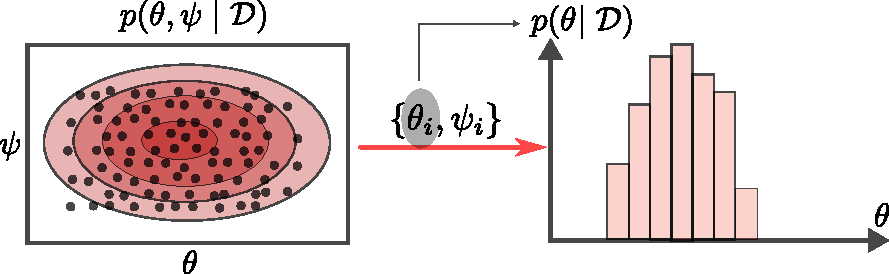
\includegraphics[width=0.7\textwidth]{figures/sota_1/fullBayes.pdf}
    \caption{A visual representation of how the \gls{fb} approach is solved in practice.}
    \label{fig:sota_1:fb}
\end{figure}

Fig.~\ref{fig:sota_1:fb} shows a visual representation of how the \gls{fb} approach is solved in practice. The joint posterior $\p{\btheta, \bpsi \mid \data}$ is sampled using \gls{mcmc} techniques to extract samples $\{(\btheta_i, \bpsi_i)\}_{i=1}^{N_s}$. The user then looks at the samples of the parameters $\btheta_i$ to estimate integrals or the posterior distribution of the parameters $\p{\btheta \mid \data}$ (for example using histograms or \gls{kde} techniques). 

\subsection{The Issue of Identifiability}

The second issue of the \gls{fb} framework is the issue of identifiability~\cite{Gramacy2015}. In this section we will show that the issue of identifiability is not a problem of the \gls{fb} framework itself, but rather a problem of the design of the model error term $z(\bx; \bpsi)$ and its prior $\prior{z \mid \bpsi}$, which, precisely because it is a prior, is the choice of the practitioner. We shall also \blue{analyze} some solutions to this issue which are compatible with the Bayesian philosophy.

The calibration problem is fundamentally unidentifiable when an infinite amount of data cannot uniquely separate the physical model $f(\bx; \btheta)$ from the discrepancy term $z(\bx)$. 

\smallskip
To demonstrate this, let $(\btheta^\star, z^\star)$ be a \gls{map} solution that perfectly matches the data generating process:

\begin{equation}
y(\bx) = f(\bx; \btheta^\star) + z^\star(\bx) \;.
\end{equation}

If we perturb the parameters by a small vector $\delta\btheta$, a first-order Taylor expansion yields:

\begin{equation}
f(\bx; \btheta^\star + \delta\btheta) \approx f(\bx; \btheta^\star) + \mathcal{J}[\delta \btheta](\bx) \;,
\end{equation}

where $\mathcal{J}$ maps the perturbation to the model's directional derivative:

\begin{equation}
\mathcal{J}[\delta \btheta](\bx) = \langle \delta\btheta, \nabla_{\btheta}f(\bx; \btheta^\star) \rangle \;.
\end{equation}

Substituting this back into the data equation gives:

\begin{equation}
y(\bx) \approx f(\bx; \btheta^\star + \delta\btheta) + \big(z^\star(\bx) - \mathcal{J}[\delta \btheta](\bx)\big)\;.
\end{equation}

Thus, the alternative pair $\big(\btheta^\star + \delta\btheta, \, z^\star(\bx) - \mathcal{J}[\delta \btheta](\bx)\big)$ explains the data equally well, provided the perturbed discrepancy remains within the function space of $z$ (typically guaranteed for flexible Gaussian Processes).

\smallskip
Unidentifiability creates posteriors that are highly sensitive to the prior $\prior{z \mid \bpsi}$~\cite{Tuo2015} and never concentrate around a single mode~\cite{hagan_2014}. For instance, if a linear model $f(x; \theta) = \theta x$ and a quadratic error term $z(x) = \psi_0 + \psi_1 x + \psi_2 x^2$ fit a true map $y = 1 + x + x^2$, infinitely many valid parameter pairs live on the line $\psi_1 = 1 - \theta$. The error term $z$ absorbs the model's output. To fix this, we must constrain $z$~\cite{hagan_2014,Plumlee2017,leoni}.

\smallskip
Previously, Hagan et al.~\cite{hagan_2014} used pointwise constraints, while Plumlee~\cite{Plumlee2017} enforced orthogonality between $z$ and the model sensitivities $\mathcal{J}[\delta \btheta]$. However, Leoni~\cite{leoni} argued that Plumlee's approach defines a ``true'' parameter value that may not be physically meaningful.

\smallskip
In a purely Bayesian framework, claiming a single ``true'' parameter value $\btheta^\star$ is flawed, especially for mis-specified models. Instead, practitioners define priors $\prior{z \mid \bpsi}$ and $\prior{\btheta}$ and let data update them. Since these priors rely on subjective choices about the underlying true map, we should debate the \textit{reasonableness} of the priors rather than the \textit{truth} of the parameters.

\smallskip
Identifiability issues occur when $\prior{z \mid \bpsi}$ is too flexible, allowing infinite equivalent modes that prevent the posterior from concentrating. We solve this by restricting the space of $z$ via a linear constraint operator $\mathcal{C}[z] = 0$.

\smallskip
For a perturbed discrepancy $z^\star(\bx) - \mathcal{J}[\delta \btheta]$ to remain valid, it must satisfy $\mathcal{C}[z^\star - \mathcal{J}[\delta \btheta]] = 0$. By linearity:

\begin{equation}
    \begin{aligned}
        \mathcal{C}[z^\star - \mathcal{J}[\delta \btheta]] &= \mathcal{C}[z^\star] - \mathcal{C}[\mathcal{J}[\delta \btheta]] \\
        &= - (\mathcal{C} \circ \mathcal{J}) [\delta \btheta]\;. \\
    \end{aligned}
\end{equation}

We define the \textit{Interaction Operator} as $\mathcal{M} = \mathcal{C} \circ \mathcal{J}$. The problem is identifiable if and only if $\mathcal{M}$ is injective, meaning $\text{Ker}(\mathcal{M}) = \{0\}$. This forces $\delta \btheta = 0$. Thus, to guarantee identifiability, the number of constraints must at least equal the number of parameters.

\subsubsection{Pointwise Constraints}

As first proposed by~\cite{hagan_2014}, pointwise constraints fix the value of the model error term and its derivatives at specific locations in the input space. For example, if we want to enforce $z(\bx_0) = 0$ and $\nabla_{\bx} z(\bx_0) = \mathbf{0}$, the interaction operator is given by,

\begin{equation}
    \mathcal{M}_{\btheta} = \begin{bmatrix} \nabla_{\btheta} f(\bx_0; \btheta)^\top \\ \nabla_{\bx} \nabla_{\btheta} f(\bx_0; \btheta)^\top \end{bmatrix} \;.
\end{equation}

We see that the identifiability of the calibration problem depends on the sensitivity of the model output to the parameters at the point $\bx_0$.

\subsubsection{Feature removal constraints} 
A similar approach to get physically meaningful parameters is to remove specific \textit{features} from the discrepancy function. Assume that we want the discrepancy to not be able to capture a shape $\phi(\bx)$ (e.g., constant offsets, linear trends), a constraint operator can be defined as:

\begin{equation}
    \mathcal{C}[z] = \langle z, \phi \rangle = \int_{\Omega} z(\bx) \phi(\bx) \, \dd \bx = 0 \;.
    \label{eq:trend_removal_constraint}
\end{equation}

The corresponding interaction operator is then given by,
\begin{equation}
    \mathcal{M}_{\btheta} = \int_{\Omega} \phi(\bx) \nabla_{\btheta} f(\bx; \btheta)^\top \, \dd \bx \;.
\end{equation}

\subsubsection{Orthogonality constraint}
The orthogonality constraint proposed by~\cite{Plumlee2017} enforces the model error term to be orthogonal to the sensitivity of the model output to the parameters. This constraint can be expressed as a feature removal constraint with $\phi_i(\bx) = \mathcal{J}_i(\bx)$. In this case the interaction operator is given by the Gram matrix of the Jacobian, $\mathcal{M}_{ij} = \int_{\Omega} \mathcal{J}_i(\bx) \mathcal{J}_j(\bx) \, \dd \bx$. The identifiability is guaranteed if the base model is sensitive to all the parameters, i.e., $\mathcal{M}$ is positive definite.

\subsubsection{Informative priors}
Finally, a different approach to inject prior beliefs on the model error term is to use informative priors $\prior{\bpsi}$ that constrain the \gls{gp} prior $\prior{z; \bpsi}$ to have specific properties. A good reference for choosing informative priors is the work of~\cite{stat_dec_th}. While this approach does not constrain the model error and therefore does not guarantee identifiability, it can still be used to inject prior beliefs on the model error term and mitigate confounding effects. Furthermore, specifying the structure of $\prior{\bpsi}$ is sometimes more intuitive than specifying the structure of the constraint operator $\mathcal{C}$.


\subsubsection{Example 1: The Simple Machine}
As a first example, we consider the simple machine example introduced by~\cite{hagan_2014}. The true system is given by $y(x) = 0.65x/(1+x/20)$, and the computer model is a simple linear function $f(x; \theta) = \theta x$. We generate 11 synthetic observations of the system at $x \in [4, 10]$ with Gaussian noise of standard deviation $\sigma_{\text{obs}} = 0.001$ (to mimic the infinite data limit). The model error term is modeled as a zero mean \gls{gp} with an \gls{rbf} covariance. Uniform priors are used for the parameters and hyperparameters. 

\smallskip
In their original work, the authors compared the results of the \gls{fb} framework with the results obtained by enforcing the discrepancy and its gradient to be zero at $x=0$. Their rationale was to recover the physical value of the parameter $\theta$ that corresponds to the slope of the true system at $x=0$. 

\smallskip
\blue{Analyzing the effectiveness of the constraints}, we can immediately see that enforcing the discrepancy to be zero at $x=0$ yields an interaction operator $\mathcal{M} = \partial_{\theta}f(x=0)$, which is $0$. This first constraint is therefore not useful. Enforcing the gradient of the discrepancy to be zero at $x=0$ yields an interaction operator $\mathcal{M} = \partial^2_{x\theta}f(x=0)$, which is $1$. This second constraint is therefore sufficient to guarantee identifiability.

\begin{figure}[htbp]
  \centering
  \begin{subfigure}[t]{0.49\linewidth}
       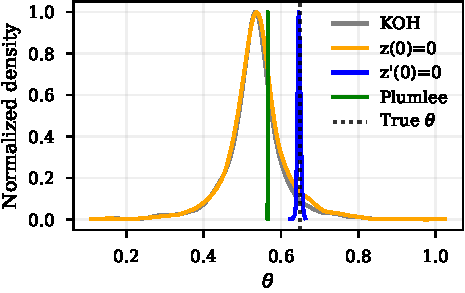
\includegraphics[width=\textwidth]{figures/sota_1/simple_machine_sigma_0.001.pdf}
    \caption{Posterior distribution of the parameter $\theta$ obtained by enforcing different constraints.}
    \label{fig:sota_1:simple_machine_posterior}
  \end{subfigure}
  \begin{subfigure}[t]{0.49\linewidth}
    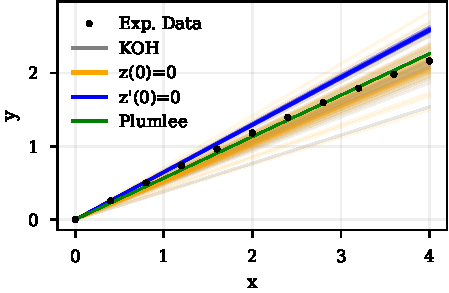
\includegraphics[width=\textwidth]{figures/sota_1/realizations_sigma_0.001.pdf}
    \caption{Posterior realizations of $f(x; \theta)$ obtained by enforcing different constraints.}
    \label{fig:sota_1:realizations}
  \end{subfigure}
  \caption{Posterior distribution of the parameter $\theta$ and posterior realizations of $f(x; \theta)$ obtained by enforcing different constraints.}
  \label{fig:sota_1:simple_machine_constraints}
\end{figure}

\blue{In Fig.~\ref{fig:sota_1:simple_machine_constraints} we show the results of the simple machine example. Fig.~\ref{fig:sota_1:simple_machine_posterior} shows the posterior distribution of the parameter $\theta$ and Fig.~\ref{fig:sota_1:realizations} shows the posterior realizations of $f(x; \theta)$. As expected, the \gls{koh} framework without constrains (and similarly the \gls{koh} framework with a constraint on the discrepancy at $x=0$) is not able to identify a single value of $\theta$ even in the limit of infinite data. Constraining the gradient of the discrepancy to be zero at $x=0$ or enforcing the orthogonality constraint yields a posterior distribution of $\theta$ that concentrates around a single value. In the first case, the value of $\theta$ corresponds to the slope of the true system at $x=0$, the \textit{physical value}, but it is not the value that minimizes the $L^2$ distance to the data. In the second case, the value of $\theta$ corresponds to the value that minimizes the $L^2$ distance to the data, but it is not the physical value of $\theta$. This example highlights how different constraints yield different definitions of the model parameters and how one should be careful when talking about \textit{true} values of the parameters.}

\subsubsection{Example 2: A nonlinear Heat Equation}
To \blue{further} highlight the effect of the constraint operator on the calibration outcome, we consider the calibration of a steady heat equation in 1D with a nonlinear thermal conductivity. The \gls{pde} is given by,

\begin{equation}
\label{eq:strong_form}
\begin{cases}
- \dfrac{d}{dx} \left( k(T) \dfrac{dT}{dx} \right) = q_0, & \text{in } \Omega, \\
T = 0, & \text{on } \partial \Omega,
\end{cases}
\qquad \text{with } \Omega = (0,1).
\end{equation}

We consider the case in which $k(T) = 1 + 0.5 T + 0.2 T^2$ is a nonlinear function of the temperature $T$ and $q_0 = 50$ is a constant heat source. We calibrate a constant model for the thermal conductivity, i.e., $k(T) = \theta$, which corresponds to a mis-specified model. We generate 20 synthetic observations of the temperature profile with a Gaussian noise of standard deviation $\sigma_{\text{obs}} = 0.01$. The model error term is modeled as a zero mean \gls{gp} with a \gls{rbf} covariance. Uniform priors are used for the parameters and hyperparameters.

\smallskip
We first consider Plumlee's approach, which enforces the model error term to be orthogonal to the sensitivity of the model output to the parameters. Using the true solution of the \gls{pde} (a simple parabolic profile) we see that this approach forces $z(x)$ to be orthogonal to parabolas proportional to $x(1-x)$. 

\smallskip
We consider a second constraint, inspired by the energy balance of the system. The total energy in the system is given by the integral of the temperature profile, $E \propto \int_0^1 T(x; \theta) \, \dd x$. Since our temperature profile is the sum of the model output and the model error term, we can rewrite the energy as $E \propto \int_0^1 f(x; \theta) + z(x) \, \dd x$. If we enforce the model error term to have zero mass, i.e., $\int_0^1 z(x) \, \dd x = 0$, we are effectively enforcing the calibrated model to be responsible for the entire energy balance in the system. This constraint can be expressed as a feature removal constraint with $\phi(x) = 1$. 

\begin{figure}[htbp]
    \centering
    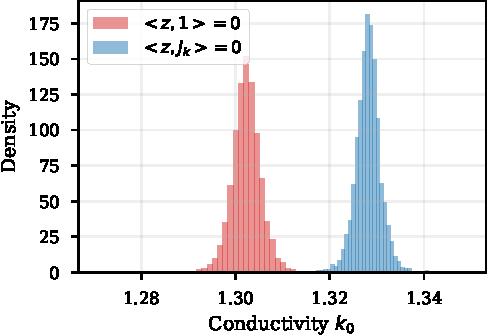
\includegraphics[width=0.5\linewidth]{figures/sota_1/heat_posterior_k0_comparison.pdf}
    \caption{Posterior distribution of the thermal conductivity $\theta$ obtained under different constraints. }
    \label{fig:sota_1:heat_informed_vs_uninformed}
\end{figure}

In Fig.~\ref{fig:sota_1:heat_informed_vs_uninformed} we show the posterior distribution of the thermal conductivity under different constraints. \blue{Both constraints yield a posterior distribution that concentrates around a single value, but the two distributions are different. Contrary to the previous example, this example highlights that there is no \textit{true} value of the parameters, as the model for the thermal conductivity is mis-specified. The choice of the model error prior determines the meaning of the inferred parameters. Enforcing the orthogonality constraint yields a higher value of the thermal conductivity, which is the one that minimizes the $L^2$ distance to the data, while enforcing the zero mass constraint yields a lower value of the thermal conductivity, which is the one that satisfies the energy balance of the system.}



\section{Beyond the Full Bayes framework: Modular approaches and their limitations}
\label{sec:sota_1:modularization}

In this section we will present modular approaches to calibration, which are a popular alternative to the \gls{fb} framework. After presenting the different approaches to modularization, we will discuss their limitations and why they are not compatible with the Bayesian philosophy. We will then lay the groundwork for the next chapter, in which we will present a novel calibration framework aimed at solving the issues of the \gls{fb} framework and the limitations of modular approaches.

\subsection{Modular Approaches}

Modular approaches to calibration are a popular alternative to the \gls{fb} framework, and are widely used by the frequentist community~\cite{freq_calibration}. First theorized by~\cite{mod_approaches}, modular approaches solve the calibration problem sequentially by first estimating the model error term (or its hyperparameters) and then conditioning the posterior of the parameters on this estimate. In our context this means that one first computes an estimate $\bar{\bpsi}$ of the hyperparameters of the model error term (for example using the \gls{map} or \gls{mle} estimator) and then conditions the posterior of the parameters on this estimate, i.e., $\p{\btheta \mid \data, \bar{\bpsi}}$.

\begin{figure}[htbp]
    \centering
    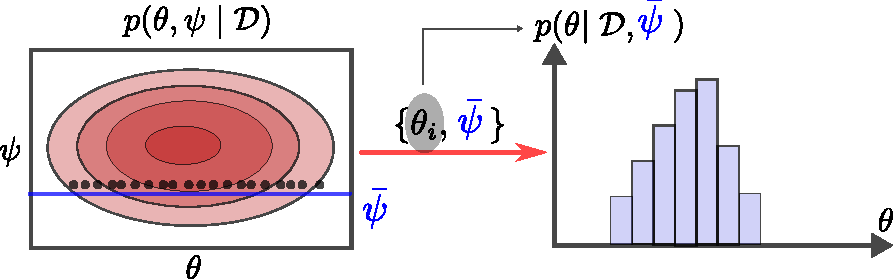
\includegraphics[width=0.7\textwidth]{figures/sota_1/modular.pdf}
    \caption{A visual representation of how a modular approach is solved in practice.}
    \label{fig:sota_1:modular}
\end{figure}

Fig.~\ref{fig:sota_1:modular} shows a visual representation of how a modular approach is solved in practice. First, one estimates the hyperparameters $\bar{\bpsi}$ of the model error term (we shall see how this can be done later), and then one samples from the posterior $\p{\btheta \mid \data, \bar{\bpsi}}$ to estimate the posterior distribution of the parameters.

\smallskip
Modular approaches are very popular in practice, since they solve the issues of the \gls{fb} framework by sampling from a posterior distribution of reduced dimension $\p{\btheta \mid \data, \bar{\bpsi}}$ instead of the joint posterior $\p{\btheta, \bpsi \mid \data}$. They also \textit{tame} the identifiability issue by fixing the model error term to a specific value $\bar{\bpsi}$, thus reducing the flexibility of the model error term and allowing the data to update the posterior distribution of the parameters $\p{\btheta \mid \data, \bar{\bpsi}}$ into a distribution that concentrates around a single mode.

We shall now present some of the most popular approaches to estimate the hyperparameters $\bar{\bpsi}$ of the model error term. 

\subsubsection{The MAP estimator}
In their original work, Kennedy and O'Hagan~\cite{koh2001_sup} proposed to fix the hyperparameters to their \gls{map} estimate,

\begin{equation}
    \psikoh = \argmax_{\bpsi} \p{\bpsi \mid \data} = \argmax_{\bpsi} \intt{\p{\btheta, \bpsi \mid \data}}\;.
\end{equation}

In this work, we will refer to this approach as the \gls{koh} method.

\subsubsection{The Maximum Likelihood estimator}
Originally proposed by~\cite{Bachoc2013}, the \gls{mle} fixes the hyperparameters to the value that maximizes the likelihood,

\begin{equation}
    \bpsi_{_\mathrm{MLE}} = \argmax_{\bpsi} \p{\data \mid \bpsi}\;.
\end{equation}

\subsubsection{The Maximum LOO Estimator}
Also proposed by~\cite{Bachoc2013}, the \gls{loo} estimator fixes the hyperparameters to the value that maximizes the \gls{loo}-\gls{cv} score,

\begin{equation}
    \bpsi_{_\mathrm{LOO}} = \argmax_{\bpsi} \sum_{i=1}^{\nobs} \log \p{y_i \mid \data_{-i}, \bpsi}.
\end{equation}

where $\data_{-i} = \{(\bx_j, y_j)\}_{j=1\ldots \nobs, j\neq i}$ is the dataset with the $i$-th observation removed. The \gls{loo}-\gls{cv} score is a popular metric to evaluate the predictive performance of a model, and it is often used to select the hyperparameters of a model.
Other techniques to estimate the hyperparameters of the model error term include the use of a validation set, the use of an iterative approach that alternates between estimating the hyperparameters and the parameters, but they all share the same philosophy of fixing the hyperparameters to a specific value $\bar{\bpsi}$ and then conditioning the posterior of the parameters on this value. We refer the interested reader to~\cite{leoni} for a more comprehensive review of the different approaches to estimate the hyperparameters of the model error term. In this work, we shall not be concerned with the specific technique used to estimate the hyperparameters, since all these techniques share the same philosophy and limitations, which we will discuss in the next section.

\subsection{A Critique of Modular Approaches}

We have seen that modular approaches are \blue{a popular alternative to the \gls{fb} framework, as they reduce the dimensionality of the posterior distribution and tame the identifiability issue. However, they suffer from severe issues that make them incompatible with the Bayesian philosophy. In this section we will discuss these issues and why they are critical to the calibration outcome.}

\smallskip
First and foremost, modular approaches are not compatible with the Bayesian framework, since they break the natural flow of uncertainty that goes from the parameters $\btheta$ to the hyperparameters $\bpsi$ and vice-versa. Fixing the hyperparameters, is equivalent to reducing their posterior distribution $\p{\bpsi \mid \data}$ to a point mass, also underestimating the posterior uncertainty of the parameters $\btheta$. To be more precise, this is not a violation of the Bayesian principle per se, as a point mass prior $\prior{\bpsi} = \delta(\bpsi - \bar{\bpsi})$ can be used to justify this conditioning and yield the same result. However, the violation of the Bayesian principle arises from the fact that the data $\data$ is used twice: once to choose the value $\bar{\bpsi}$ and once to condition on it. Or in other words, a point mass prior such the one above depends on the data. This is a clear violation of strict subjective Bayesian principles, though this practice is formally recognized in statistical literature within the framework of Empirical Bayes or Type-II Maximum Likelihood~\cite{mod_approaches, uq_theory}. This is otherwise understood from the fact that any estimation of the hyperparameters $\bar{\bpsi}$ from the data $\data$ comes with its own uncertainty, which is not accounted for in the modular approaches. If a practitioner has a strong prior belief on the value of the hyperparameters $\bpsi$, a modular approach is valid, but if no prior belief is available, then either the \gls{fb} framework should be used, or one needs to switch to a frequentist approach directly.

\smallskip
It is important to remark that if identifiability is an issue, the modular approach is not a valid solution, and we have shown valid Bayesian solutions to this issue in the previous section. 

\smallskip
One could argue that we are being too harsh on modular approaches. Indeed, even a \gls{fb} approach requires a prior distribution $\prior{\bpsi}$ but this prior may also be parameterized by some hyper-hyperparameters $\boldsymbol{\xi}$, i.e. $\prior{\bpsi} = \prior{\bpsi \mid \boldsymbol{\xi}}$ (for example if we use a normal prior $\boldsymbol{\xi}$ could represent the mean and variance of the normal distribution). Why do we fix these hyper-hyperparameters to specific values instead of putting a prior $\prior{\boldsymbol{\xi}}$? Aren't we also violating the Bayesian principle in this case? Strictly speaking, no, assuming that the hyper-hyperparameters $\boldsymbol{\xi}$ are fixed a priori and do not depend on the data $\data$, we are not violating the Bayesian principle. Furthermore, there are techniques to specify the hyper-hyperparameters $\boldsymbol{\xi}$ that are statistically rigorous and meaningful, such as those described in~\cite{stat_dec_th}. Those techniques are not available for the hyperparameters $\bpsi$ of the model error term, since they are data-dependent or problem specific. 

\smallskip
\blue{To illustrate the issues arising from modular approaches, let's consider} the case in which the model error term is modeled as a \gls{gp} with an \gls{rbf} covariance. The hyperparameters of the model error term are the lengthscale and variance of the \gls{rbf} covariance, which control the smoothness and amplitude of the model error term. Those parameters can't generally be fixed a priori, and their estimation from the data is critical to the calibration outcome. Furthermore, the uncertainty on the hyperparameters of the model error term is critical and should be accounted for in the posterior distribution of the parameters $\btheta$. 


\begin{figure}[htbp]
    \centering
    \begin{subfigure}{0.48\textwidth}
        \centering
        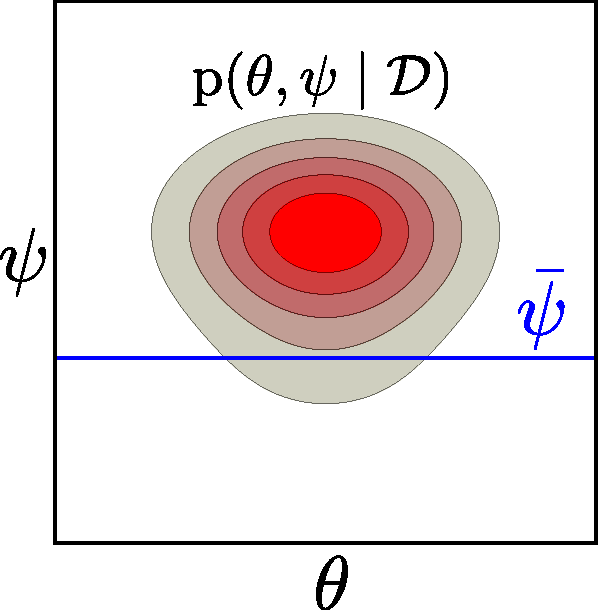
\includegraphics[width=0.6\textwidth]{figures/sota_1/Avocado.pdf}
        \caption{\blue{Example 1: Uncertainty on the hyperparameters $\bpsi$ requires careful selection of the value $\bar{\bpsi}$ to avoid underestimating the uncertainty on the parameters $\btheta$.}}
    \end{subfigure}
    \hfill
    \begin{subfigure}{0.48\textwidth}
        \centering
        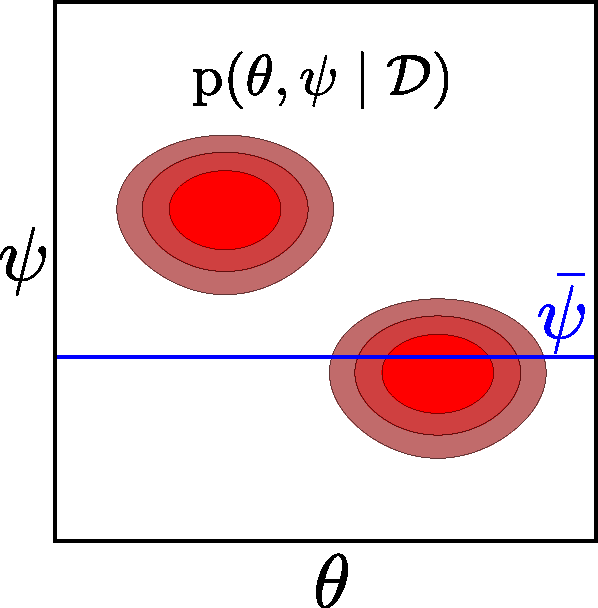
\includegraphics[width=0.6\textwidth]{figures/sota_1/doubleExp.pdf}
        \caption{\blue{Example 2: Bimodal posterior distribution of the parameters $\btheta$ arises when different values of $\btheta$ require different values of $\bpsi$ to explain the data.}}
    \end{subfigure}
    \caption{\blue{Two examples that highlight the limitations of modular approaches.}}
    \label{fig:limitations}
\end{figure}

\blue{In Fig.~\ref{fig:limitations} we show two examples that highlight the limitations of modular approaches. In the left panel, we show what happens when a modular approach is used in a scenario where the hyperparameters $\bpsi$ are uncertain. In this case, fixing $\bpsi$ to a specific value $\bar{\bpsi}$ can yield a posterior distribution of the parameters $\p{\btheta \mid \data, \bar{\bpsi}}$ that is much more concentrated than the true posterior $\p{\btheta \mid \data}$, thus underestimating the uncertainty on the parameters. In the right panel, we show a common issue in calibration with model error, which is the fact that different values of $\btheta$ require different values of $\bpsi$ to explain the data. In this case, fixing $\bpsi$ to a specific value $\bar{\bpsi}$ will generally pick a single mode of the posterior distribution of the parameters, which can lead to biased estimates of the parameters and underestimation of their uncertainty.}


\smallskip
\blue{In conclusion, modular approaches are not compatible with the Bayesian philosophy. Although they are a popular way to reduce the dimensionality of the posterior distribution and to tame the identifiability issue, they suffer from severe limitations that can lead to biased estimates of the parameters $\btheta$ and underestimation of their uncertainty, calling for more rigorous approaches to model error selection and estimation.}

\subsection{Adaptive Estimation of the Hyperparameters}

On the one hand, we have seen that modular approaches are not compatible with the Bayesian philosophy and one needs to use the \gls{fb} framework to properly account for the uncertainty on the hyperparameters $\bpsi$ of the model error term. On the other hand, we have seen that sampling from the joint posterior $\p{\btheta, \bpsi \mid \data}$ is a challenging task, especially when the dimension of $\bpsi$ is large. 

\smallskip
\blue{The only way to rigorously reduce the dimensionality of the posterior distribution is to marginalize the hyperparameters $\bpsi$ and sample from the marginal posterior $\p{\btheta \mid \data}$. Such an approach would have the same advantages of modular approaches, as it reduces the dimensionality of the posterior distribution, but it would also be compatible with the Bayesian philosophy, as it would rigorously account for the uncertainty on the hyperparameters $\bpsi$. In order to sample from the marginal posterior $\p{\btheta \mid \data}$, one needs to integrate out the hyperparameters $\bpsi$ from the joint posterior $\p{\btheta, \bpsi \mid \data}$, which is generally a challenging task. However, if one can find a good approximation of the marginal posterior $\p{\btheta \mid \data}$, one can sample from this approximation to estimate the posterior distribution of the parameters $\btheta$.}

\begin{figure}[htbp]
    \centering
    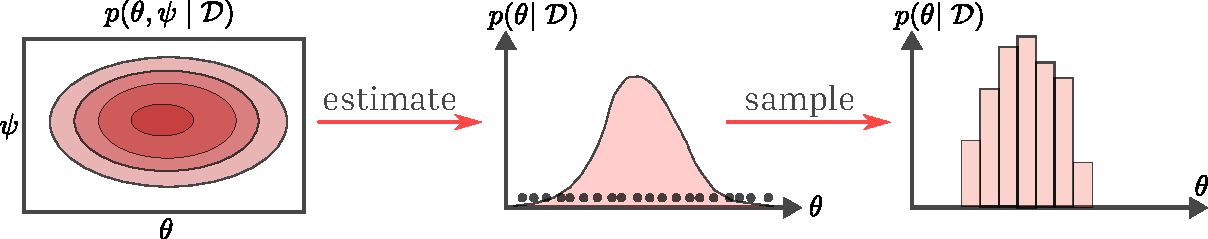
\includegraphics[width=\textwidth]{figures/sota_1/cmp.pdf}
    \caption{A visual representation of the proposed approach. We first approximate the marginal posterior $\p{\btheta \mid \data}$ and then sample from this approximation.}
    \label{fig:sota_1:cmp}
\end{figure}

\blue{In Fig.~\ref{fig:sota_1:cmp} we show a visual representation of the proposed approach. We first approximate the marginal posterior $\p{\btheta \mid \data}$ and then sample from this approximation to estimate the posterior distribution of the parameters $\btheta$. Such an approach was originally proposed by~\cite{fmp, leoni} and is known as the \gls{fmp} method. The \gls{fmp} method is a modular approach that uses an \textbf{adaptive estimator} of the hyperparameters $\bpsi$ that depends on the parameters $\btheta$. This is in contrast to the modular approaches presented in the previous section, which use a fixed estimator of the hyperparameters $\bar{\bpsi}$ that does not depend on the parameters $\btheta$. The estimator of the hyperparameters $\bpsi$ used in the \gls{fmp} method is the \gls{map} estimator, which is given by,}

\begin{equation}
    \psimap = \argmax_{\bpsi} \p{\bpsi, \btheta \mid \data} \;.
    \label{eq:sota_1:fmp}
\end{equation}

Conditioning the likelihood on this estimate \blue{yields the following approximation of the marginal posterior $\p{\btheta \mid \data}$,}

\begin{equation}
    \approxp{\fmp}{\btheta \mid \data} \propto \p{\data \mid \btheta, \psimap} \prior{\btheta} \;.
    \label{eq:sota_1_pfmp}
\end{equation}

\blue{Notice that in Eq.~\eqref{eq:sota_1:fmp} the estimator $\psimap$ depends on the parameters $\btheta$, which is the key difference with respect to the modular approaches presented in the previous section. The \gls{fmp} method has been applied to various problems in the literature, including the calibration of a complex multiphase flow model~\cite{leoni}. The results show a good agreement with the \gls{fb} framework~\cite{leoni}, but with some limitations.}

\smallskip
\blue{In particular, the authors of~\cite{leoni} show that the \gls{fmp} method can identify all modes of the posterior distribution of the parameters $\btheta$, but fails to correctly assign the correct probability mass to each mode. This is due to the fact that the \gls{fmp} method uses a point estimate of the hyperparameters $\bpsi$ for each value of $\btheta$, which does not account for the uncertainty on $\bpsi$. Furthermore, in Eq.~\eqref{eq:sota_1_pfmp} the prior of the hyperparameters $\prior{\bpsi}$ is not accounted for. In their original work, the authors only considered a bounded uniform prior on the hyperparameters $\bpsi$, but in general, the prior of the hyperparameters $\prior{\bpsi}$ can be informative and should be accounted for in the approximation of the marginal posterior $\p{\btheta \mid \data}$.}

\smallskip
\blue{Overall, the above-mentioned issues of the \gls{fmp} method arise from the fact that Eq.~\eqref{eq:sota_1_pfmp} is a good approximation of the marginal posterior $\p{\btheta \mid \data}$ only under very stringent hypotheses. In particular, the approximation is valid only if the posterior distribution of the hyperparameters $\p{\bpsi \mid \data, \btheta}$ is a point mass distribution centered at $\psimap$ (no uncertainty on $\bpsi$) and that $\psimap$ is weakly dependent on $\btheta$~\cite{fmp}. In practice, these hypotheses are rarely satisfied, and the approximation of the marginal posterior $\p{\btheta \mid \data}$ given by Eq.~\eqref{eq:sota_1_pfmp} can be poor. Furthermore, when considering priors on the hyperparameters $\prior{\bpsi}$, with a large support, the \gls{fmp} approximation results in a degenerate distribution, which can't be sampled using standard \gls{mcmc} methods.}


\smallskip
\blue{The future developments of the next chapter will be to propose a new set of assumptions on the calibration problem that will allow us to derive a novel approximation of the marginal posterior $\p{\btheta \mid \data}$ that solves the issues of the \gls{fmp} method.}

